\chapter{Results}
\label{cha:results}

\todo{some intro}

\section{Architecture of the proposed solution}
\label{sec:architecture}

\Cref{fig:architecture} presents the overview of main components of the solution. First, the data about locations used for micro-location purposes, held in human heads needs to be digitized into computer-readable maps in OpenGIS format.

\todo{finish}

\begin{figure}
	\centering
	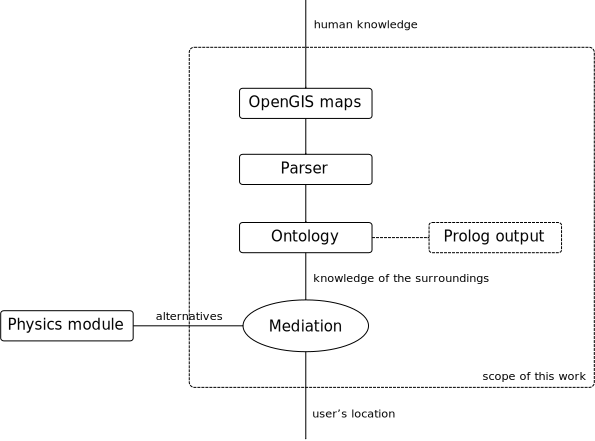
\includegraphics[width=\textwidth]{architecture}
	\caption{Architecture of the proposed solution (own work).}
	\label{fig:architecture}
\end{figure}

\section{OpenGIS maps}

\section{Ontology}

Supports optional export to a Prolog-like format for further research.

\section{Physics-based module for providing alternative possible user locations}
\label{sec:physics-module}

To get a few alternative location (an input to the mediation process, ``where the user might be''), an external physics-based module is used. The one used currently is the subject of work of Bobek and Grodzki among others, and more about it can be read in \cite{bobek2015indoor, Koeping2015indoor}. Therein, details of mathematical models used are presented.

The basic idea is to use two sources of data. If inferred locations occupy more than one room, mediation is triggered. The sources are:

\begin{itemize}
	\item dead-reckoning (pedometer) using data from various motion sensors of a device (accelerometer, gyroscope) and
	\item strength of signals received from iBeacon-compatible transmitters placed in rooms.
\end{itemize}

Dead-reckoning (also known as ``inertial measurements'') works by changing the model's idea of user's location, incrementally adding and subtracting small changes to it (steps in this case). Amounts of these changes are inferred based on data coming from motion sensors of a devices using a mathematical model. As Köping et al. state in \cite{Koeping2015indoor}, ``We model the indoor localization problem as a recursive density estimation problem, which can be estimated by employing the Bayesian framework, namely particle filters.''

The idea for using beacons in the module is to make an assessment about distances to nearby transmitters based on signal strength and RSSI (one case of the law of inverse squares, see \cref{eq:inverse-sq} and \cref{sec:existing-uloc}). Arguably, this can be seen as somewhat of a misuse of the iBeacon technology. Manufacturers generally speak of only \emph{three} recognizable levels of ``interaction'' with the beacon (based on signal strength): \begin{itemize}
 	\item receiver being in very close proximity to the transmitter,
 	\item receiver being in the same room,
 	\item no interaction at all.
 \end{itemize}
 
Matyasik et al. claim that the RSSI-to-distance-based approach works, however, \emph{only under laboratory conditions} \cite{Matyasik:iBeacon, Matyasik:iBeacon:slides}. As iBeacons use extremely low energy to transmit the signal, even a single person walking across the room while taking the measurement---or even someone playing with the smartphone during the measurement---can influence it so negatively, that any information inferred about the distance to the signal's source cannot be reliably trusted.

\section{The process of mediation}

The shortcomings of iBeacons and dead-reckoning (\cref{sec:physics-module}) encourage the use of some additional data source. In this work, mediation is proposed.

\todo{how is intelligibility achieved?}

\section{User Experience}
\label{sec:user-experience}
